\documentclass{school-22.211-notes}
\date{February 29, 2012}

\begin{document}
\maketitle

\topic{Dilution Cross Section/Dilution Factor}
In an infinite homogeneous medium with one resonance absorber and one moderator,  we write removal rates equals scattering rates, 
\begin{align}
\left[ N_r \sigma_r (u) + N_m \sigma_m (u) \right] \phi (u) &= \int_{-\infty}^u N_m \sigma_m (u') \phi(u') P(u' \to u) \du' \\ 
&= N_m \sigma_m \int_{-\infty}^u \phi(u') P(u' \to u) \du' \\
&= N_m \sigma_m C \\
\phi(u) &\propto \frac{N_m \sigma_m}{N_r \sigma_r(u) + N_m \sigma_m} \\
\phi(u) &\propto \frac{ \frac{N_m}{N_r} \sigma_m}{\sigma_r(u) + \frac{N_m}{N_r} \sigma_m}  \label{flux-shape}
\end{align}
In the above derivation we made two assumptions:
\begin{itemize}
\item The moderator's xs is independent of energy near resonances. For almost any moderators we can pick, the assumption that the elastic scattering xs is constant is valid in the thermal range as in Figure~\ref{moderator-sigma-s}. 
\item $\int \phi(u') P(u' \to u) \du'$ is constant. We know that the flux above the resonance is 1/E and hence constant in lethargy. If we assume scattering into the resonance comes from this constant lethargy region, then the resonance lethargy is constant as well. 
\end{itemize}
\begin{figure}
  \centering
  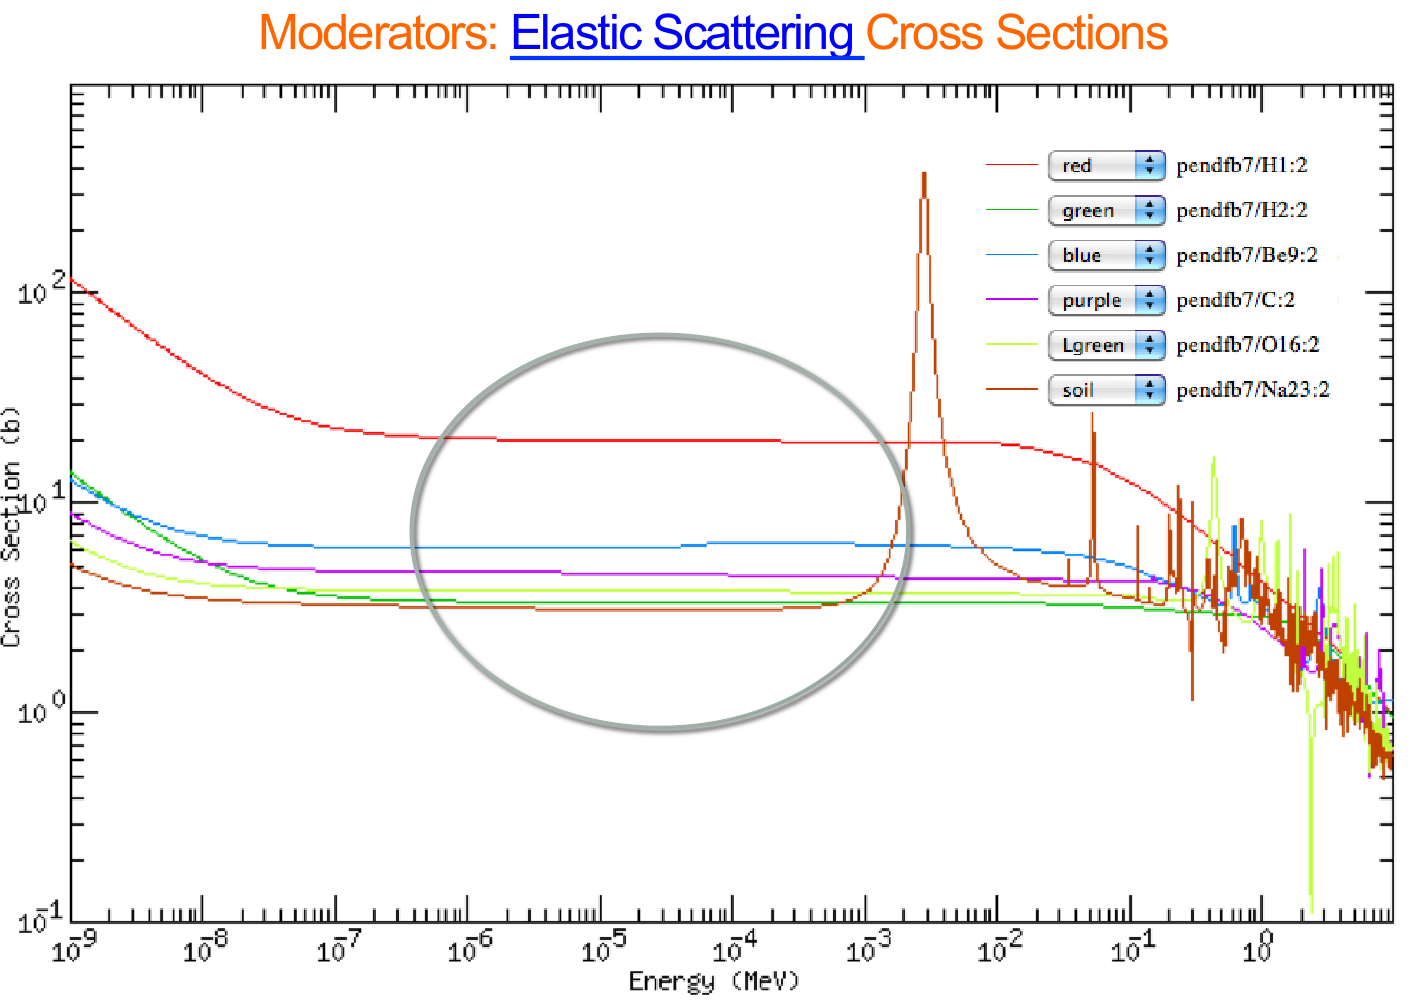
\includegraphics[width=4in]{images/moderator-sigma-s.png}
  \caption{Moderator Elastic Scattering Cross Sections} \label{moderator-sigma-s}
\end{figure}
Eq.~\ref{flux-shape} suggests that \textit{in infinite medium the flux shape near resonance depends only on the ratio of the number density of the moderator to the resonance absorber and the moderator cross section.} But once we move into a finite medium or we take into account leakage, then the absolute number densities are needed.
 
To capture the ratio of number densities and the moderator cross section, we define \hi{dilution cross section} as,
\eqn{ \boxed{ \sigma_d = \frac{N_m \sigma_m}{N_r} } }
Then the flux shape near resonance is,
\eqn{ \boxed{ \phi(u) \propto \frac{\sigma_d}{\sigma_r + \sigma_d} } }
This flux shapes let us to compute approximated effective RI. Recall RI is defined as, $\RI = \int \sigma_r (u) \du$. Then the approximated effective RI is,
\eqn{ \boxed{ \RI_{\eff} = \int \sigma_r(u) \frac{\sigma_d}{\sigma_r + \sigma_d} \du }  }
Two extremes of $\RI_{\eff}$ and $\sigma_d$:
\begin{itemize}
\item As $\sigma_d \to \infty$, the entire media is moderator, we reach the limit of infinite dilute resonance absorption appears, and $\RI_{\eff} \to \RI$;
\item As $\sigma_d \to 0$, analytically our assumptions do not hold true any more, but the MC is true that as $\RI_{\eff} \to 0, \phi \to 0$ as seen in Figure~\ref{dilution-factor-increase}. 
\end{itemize}
Figure~\ref{dilution-factor-increase} is generated from effective RI of MC calculations at 300K with half a million neutrons, 2 barns hydrogen 1/v absorber. It illustrates that, a) the dilution ratio U/H is related with dilution xs $\sigma_d$ such that they are inversely proportional; b) as the fraction of \ce{^{238} U} increases, U/H increases, $\sigma_d$ decreases, more absorption happens during resonance, hence more flux dips on the spectrum plot and smaller effective RI values in the resonance range. That is, \textit{RI are very dependent on the density of resonant materials.}
\begin{figure}
  \centering
  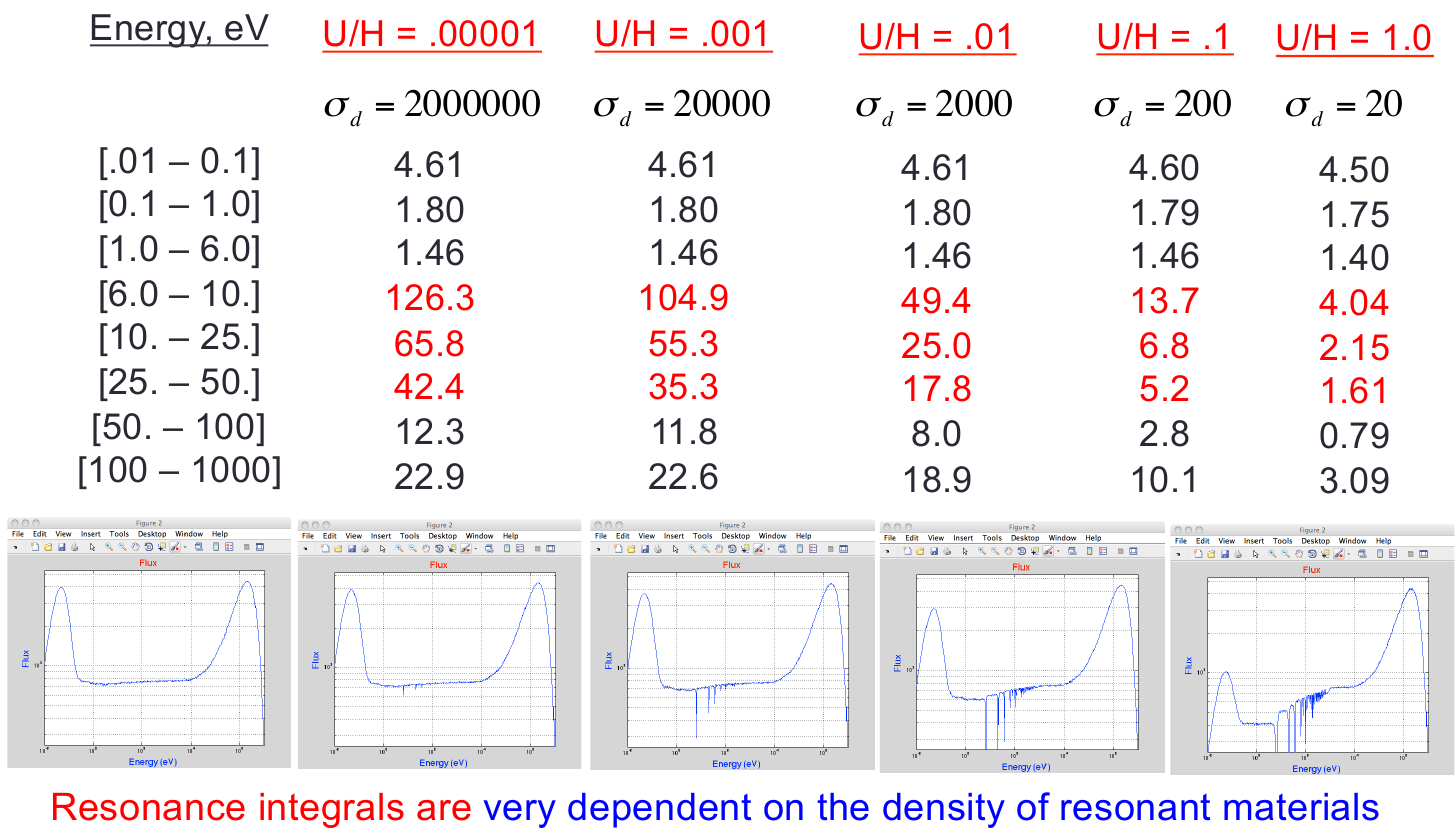
\includegraphics[width=2in]{images/dilution-factor-increase.png}
  \caption{Spectrum Resonance Dips More As U/H Increases and Dilution Cross Section Decreases} \label{dilution-factor-increase}
\end{figure}


The scattering down to resonance is independent of the resonance. In another word, if the spectrum above a resonance returns to 1/E as in Figure~\ref{1overE}, the group cross sections will be independent of higher energy absorptions. 
\begin{figure}
  \centering
  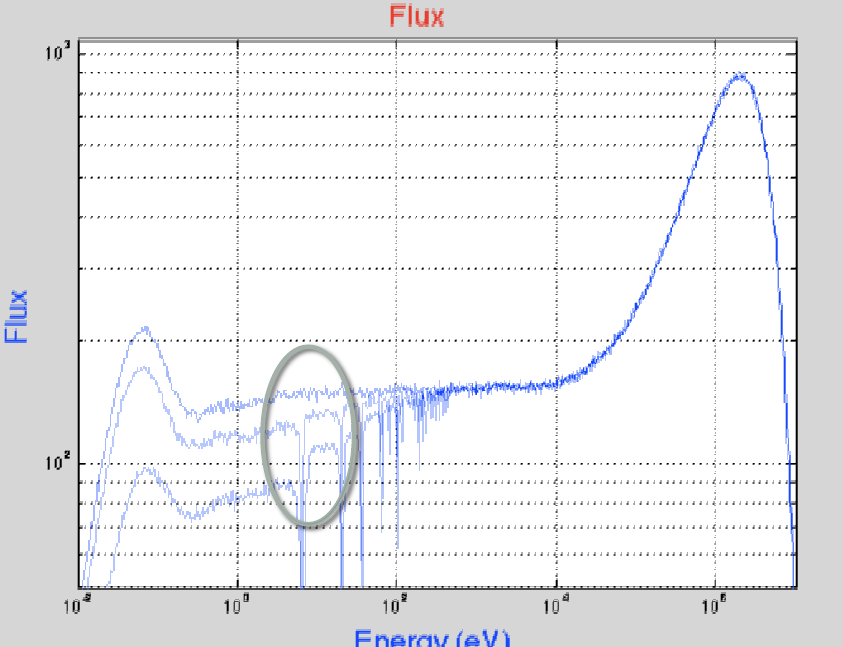
\includegraphics[width=3in]{images/resonance-1-over-E.png}
  \caption{The 1/E Spectrum Above A Resonance Suggests Group XS Independent Of Higher Energy Absorption} \label{1overE}
\end{figure}


\lecture{Analytical Derivation of Resonance Approximations}
\topic{Summary: Reuss Ch 8 Resonance Methods (FIXME)}

\topic{Wide Resonance Approximations}
The wide resonance approximation is: 
\begin{align}
\RI_{\eff} &= \int \sigma_r(u) \frac{\sigma_d}{\sigma_r(u) + \sigma_d} \du \\
&= \ln \left(\frac{E_2}{E_1} \right) \frac{ \int \sigma_r(E) \frac{\sigma_d}{\sigma_r(E) + \sigma_d} \frac{1}{E} \dE}{ \int \frac{\sigma_d}{\sigma_r(E) + \sigma_d} \frac{1}{E} \dE}
\end{align}
Notice wide resonance approximation $\RI_{\eff}$ only depends on cross sections: $\sigma_d$ is assumed to be based on material composition of the reactor, and $\sigma_r(E)$ are from libraries. There is no need for flux spectrum. 

The wide resonance approximation says that we ignore scattering of U238 because its width is large compared with the approximately 1\% energy it can lose upon scattering. To improve this approximation, sometimes people use the potential scattering of 11.39 barns. 

Wide resonance approximations match direct MC results near infinite dilution. 

\topic{Narrow Resonance Approximations}
Narrow resonance approximations assume the opposite of the wide resonance approximation, that the neutron is going to be out of the resonance upon one scattering. This approximation is good for higher energy. For instance, at 100 keV, scattering lose 1 keV, which is larger than the 25 eV spacing of \ce{^{238}U}. 

However, the results on the slides come out to be that narrow resonance approximation is not really any better than the wide resonance approximation at higher energy, so there must be some other physics going on. 


\topic{Resonance Escape Probability}
\begin{align}
p &= \exp \left( - \frac{N_R \RI_{\eff}}{\xi \Sigma_m} \right)  = \exp \left( - \frac{\RI_{\eff}}{\xi \sigma_d} \right)
\end{align}
The equation here is an approximation. And for hydrogen systems, we know $\xi \to 1$, hence the resonance escape probability becomes:
\eqn{ p = \exp \left( - \frac{\RI_{\eff}}{\sigma_d} \right) }
That is, \textit{p only depends on effective RI and dilution cross section.} For instance, in a hydrogen system with $\sigma_d = 200$, we can tabulate the p values as in Table~\ref{p-values}. The last entry tells us that \textit{about 20\% of neutrons are absorbed in U238 resonances.}
\begin{table}
  \centering
  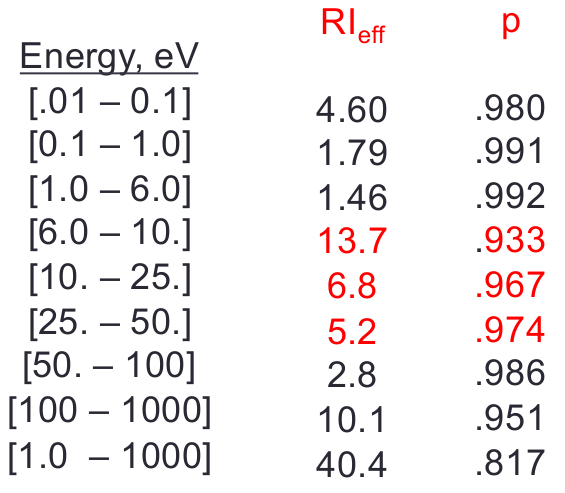
\includegraphics[width=4in]{images/resonance-escape-probability.png}
  \caption{Resonance Escape Probability For A Hydrogen System} \label{p-values}
\end{table}

\topic{NJOY Modeling of Resonance Parameters}
The normal procedure for generating multi-group xs in a code like NJOY includes:
\begin{enumerate}
\item use code to Doppler broaden cross sections for each resonance isotope for range of temperatures (eg, 300, 600, 900, 2000K); 
\item use code to apply the narrow or wide resonance models for a range of dilution xs (eg, 20000, 2000, 200, 20 barns); 
\item edit RIs or multi-group xs for your desired energy structure; 
\item build tables of xs vs. dilution xs and temperature;
\item for downstream computations, interpolate for the dilution cross section and temperature of each material in the simulation to obtain accurate multigroup cross sections for that specific applications. 
\end{enumerate}
Note that tables are general and do not have to be computed. 

A better procedure for generating multi-group cross sections includes:
\begin{enumerate}
\item the same;
\item use code to solve real neutron slowing down problem for a range of dilution cross sections (eg, 20000, 2000, 200, 20 barns);
\item consider including a mix of resonance absorbers to make the spectrum as appropriate to the desired application as possible;
\item the same;
\item the same;
\item the same.
\end{enumerate}


\topic{Homogeneous Self-Shielding Methods}

\topic{Heterogeneous Geometry Resonant Approximations}

%%%%%%%%%%%%%%%%%%%%%%%%% Qualify Exam Start %%%%%%%%%%%%%%%%%%%%%%%%%%%%
\lecture{Facts For Qualify Exam}
\begin{enumerate}
\item Flux = $\frac{n}{\cm^2 \s}.$

\item Fast flux in hydrogen is around $10^{14}$ n/cm$^2$s, and on the order of $10^{12}$n/cm$^2$s for thermal flux. 

\item U235 fission xs at 0.1 eV is about 200 barns; Pu239 fission xs is about 500 barns. In thermal reactors, Pu absorption should be about twice that of uranium. 

\item Capture cross-section as in Figure~\ref{capture-xs}: 
\begin{figure}
  \centering
  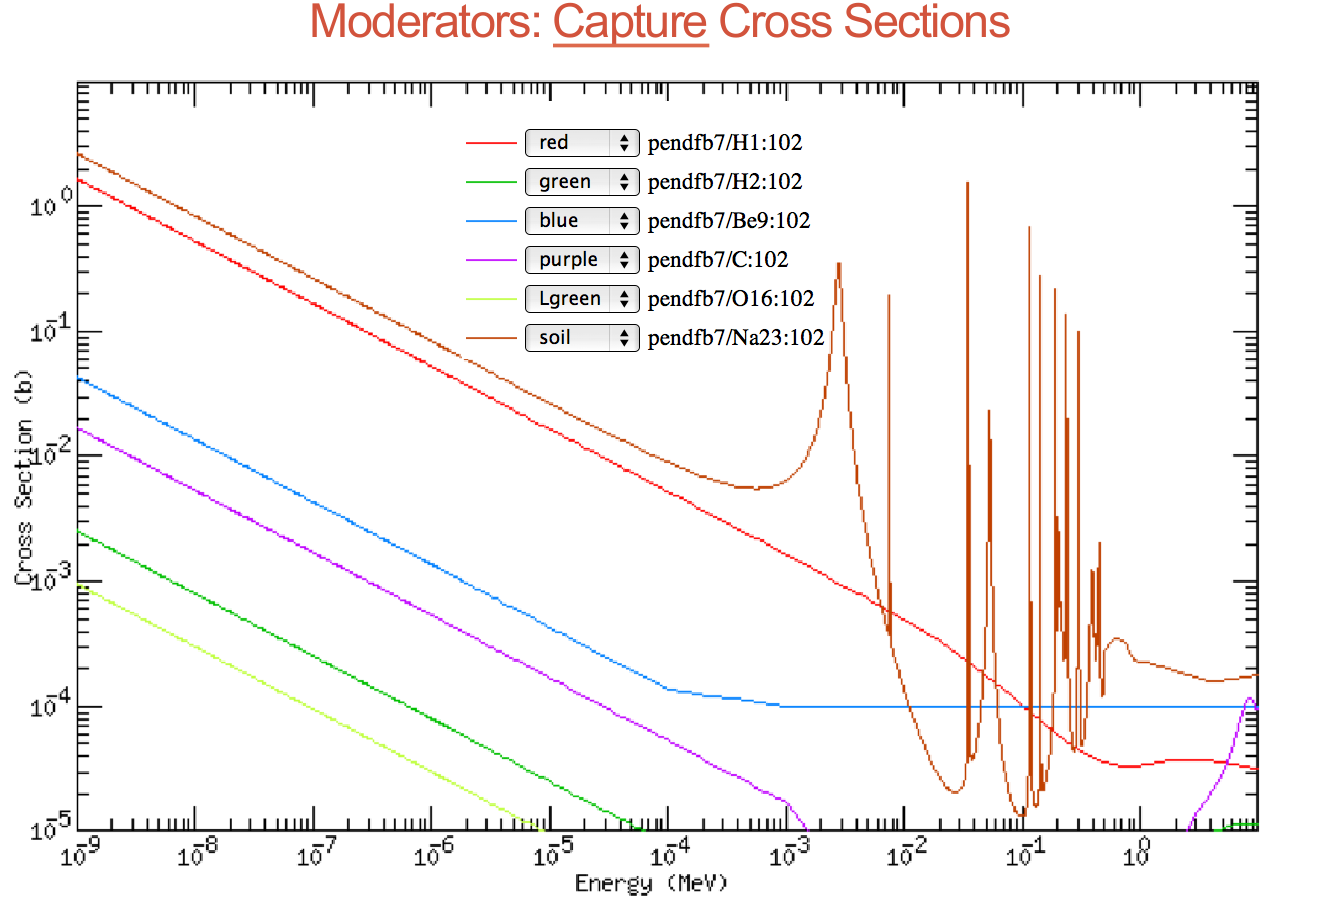
\includegraphics[width=4in]{images/capture-xs.png}
  \\
  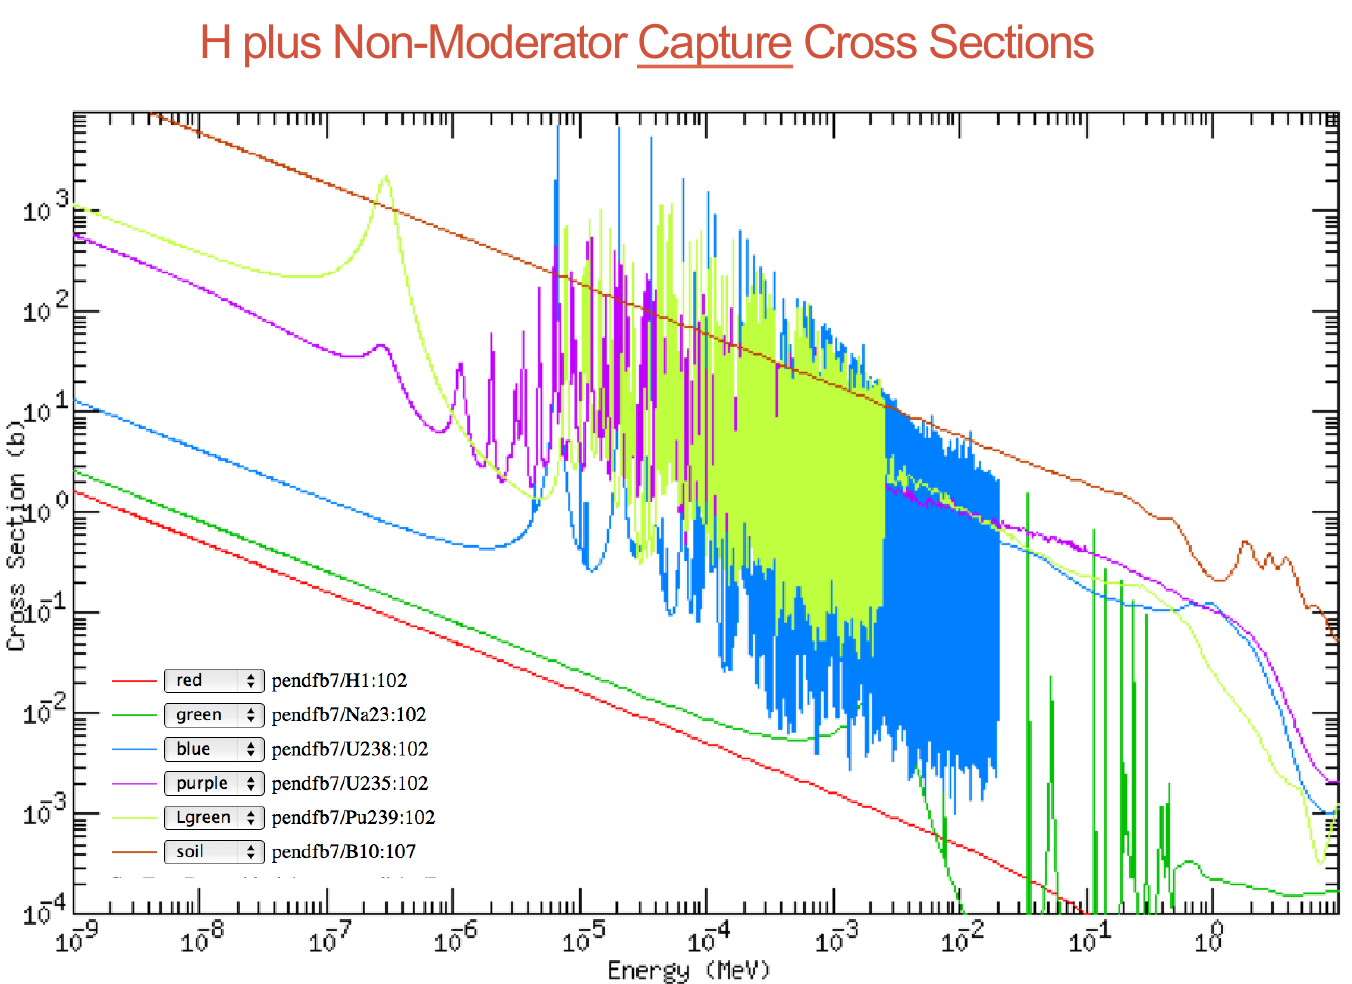
\includegraphics[width=4in]{images/capture-xs-2.png}
  \caption{Capture Cross Section} \label{capture-xs}
\end{figure}
\begin{enumerate}
\item H has no resonance; it has the highest scattering xs in LWR, so we can ignore any other isotopic's neutron scattering.   
\item Na has a huge resonance in 23 keV, and more resonances at higher energies because it is a heavy isotope.
\item Near zero energy,
\eqn{ \sigma(E\to 0) = }
\item Resonance at 6 to 7 eV: U238. 
\item U235's thermal elastic xs is larger than 238's, and they both have resonance around the same range.   
\item A small resonance at .3 eV: Pu239 (its signiture is a super low energy scattering xs). 
\end{enumerate}

\item Given an unknown material type, all we care is to count the nucleus density of each material and look at it's xs. 
\item Average fission neutron energy: 2 MeV; average peak fission energy: 1 MeV; see fission sepctrum. 

\item Core decay heat after 1 day is about 1\% rated. 


\end{enumerate}
%%%%%%%%%%%%%%%%%%%%%%%%% Qualify Exam End %%%%%%%%%%%%%%%%%%%%%%%%%%%%



\end{document}
